\chapter{Implementation}
It is now time to set up FlowVisor. In this chapter we will show two different setups.
\begin{enumerate}
    \item \textbf{Port Slicing}. A simple configuration to start things off.
    \item \textbf{IP Address Slicing}. A more complex example with more applications on a real production environment.
\end{enumerate}

FlowVisor is only configurable through the command line, so the implementations for each scenario will consist of shell scripts. Apparently FlowVisor's team of developers wanted to add a more user friendly interface, but it never came to fruition as the development had a sudden stop in 2013.

\section{First Time FlowVisor Setup}
Before we can implement any scenario, we must go through the installation and initial configuration process.

\subsection{Installation}
Right now, after going through Chapter \ref{chapter:environment}, we have a virtual machine with Mininet. We do not even have FlowVisor installed. So first things first, we need to install FlowVisor. There is no FlowVisor package on the Debian repository, so we have to run some extra commands in order to install it. Thankfully, this process is explained in the FlowVisor's Github wiki \cite{flowvisor_github}.
\begin{enumerate}
    \item Download the public GPG key for their own repository. 
    \begin{lstlisting}
    $ wget http://updates.onlab.us/GPG-KEY-ONLAB
    \end{lstlisting}
    
   \item Install the GPG key. 
    \begin{lstlisting}
    $ sudo apt-key add GPG-KEY-ONLAB
    \end{lstlisting}
    
    \item Add their repository, \textit{deb http://updates.onlab.us/debian stable/}, to the \textit{/etc/sources.list} file.
    
    \item It is now possible to install the FlowVisor package from the repository using the package manager.
    \begin{lstlisting}
    $ sudo apt-get update && sudo apt-get install flowvisor
    \end{lstlisting}
\end{enumerate}

Alternatively, it is also possible to install FlowVisor directly from the GitHub repository. Note that, in this case, it is necessary to have the \textit{git} package installed.
\begin{lstlisting}
    $ git clone git://github.com/OPENNETWORKINGLAB/flowvisor.git
\end{lstlisting}

While this last method may look simpler, it is far more cumbersome than the first alternative. When installing directly from GitHub we have to take care of some additional nuances, like FlowVisor requiring its own user, which makes it much more prone to error and misconfiguration.

\subsection{Configuration}
The main utility for configuring FlowVisor is called \textit{fvconfig}, and it is installed along the FlowVisor binary. To see every command available check the manual. While the manual is very useful, it is all we got when it comes to the documentation of \textit{fvconfig}. 
 \begin{lstlisting}
    $ man fvconfig
\end{lstlisting}

The first thing we have to do is to generate a template configuration, which is almost good enough by itself. It is important to know that \textit{fvconfig} needs be run as the \textit{flowvisor} user.
 \begin{lstlisting}
    $ sudo -u flowvisor fvconfig generate /etc/flowvisor/config.json
\end{lstlisting}

To make the implementation more manageable, we will set a blank password when asked for one. This is, after logging into \textit{sudo}, whose default password is \textit{mininet}.

Next up, we can initialize FlowVisor.
 \begin{lstlisting}
    $ sudo /etc/init.d/flowvisor start
\end{lstlisting}

Alternatively, we can also use \textit{service}.
 \begin{lstlisting}
    $ sudo service flowvisor start
\end{lstlisting}

Another utility that comes packaged with the FlowVisor binary is \textit{fvctl}, which is used to interact with the hypervisor itself once it is running. With this utility, the first thing we do is enable the topology controller.
 \begin{lstlisting}
    $ fvctl -n set-config --enable-topo-ctrl
\end{lstlisting}

The \textit{-n} flag is used when have not set a password for FlowVisor. If a password has been set, then it is necessary to type it after running the command or pass a file that contains the password using the \textit{-f} flag. After running this command we have to restart FlowVisor. 
\begin{lstlisting}
    $ sudo /etc/init.d/flowvisor restart
\end{lstlisting}

At this point, FlowVisor should be up and running, ready to connect to our Mininet network. By default, FlowVisor listens to incoming connections on port 6633. Technically, we should specify this port on the remote controller when creating the Mininet network, but Mininet tries to connect by default to localhost on port 6653 and then falls back to port 6633 if 6653 is not available. So, in practice, we do not have to specify the remote controller port on Mininet. 

\section{FlowVisor Syntax Overview}
When using FlowVisor, there are two main elements we have to work with: \textbf{slices and flowspaces.}

\subsection{Slices}
A slice is a subset of the physical underlying network. Effectively, a slice is a virtual network. Each slice is assigned to a different controller, this is what enables the possibility of offering different services with different constraints within the same physical network. To create a slice we use the \textit{add-slice} command.
\begin{lstlisting}
    $ fvctl -n add-slice example tcp:localhost:6666 admin@example
\end{lstlisting}

Where:
\begin{itemize}
    \item \textbf{example}. Name of the slice.
    \item \textbf{tcp}. Transport protocol.
    \item \textbf{localhost}. IP address where the controller lives. In this case it is in the same machine as FlowVisor.
    \item \textbf{6666}. The port where the controller is listening.
    \item \textbf{admin@example}. Contact information of the person responsible for that slice.
\end{itemize}

When running the command, the user is prompted to enter a password. Again, to avoid extra complexity, we will leave it blank.

To remove a slice, the appropriate command is \textit{remove-slice}.
\begin{lstlisting}
    $ fvctl -n remove-slice example
\end{lstlisting}

To list the existing slices, \textit{list-slices}. Note that there is always a main slice called \textit{admin}.
\begin{lstlisting}
    $ fvctl -n list-slices
\end{lstlisting}

There are more commands related to slices. To see all of them, check the manual for \textit{fvctl}.

\subsection{Flowspaces}
Once a slice is created, it is virtually useless unless the hypervisor, i.e., Flowvisor, decides to send packets to the slice. Flowspaces allow the hypervisor to know to which controller a certain packet belongs to. A flowspace is nothing more than a set of rules for a packet to be matched against. Depending on those matches, the hypervisor determines the appropriate slice. To create a flowspace, we use the \textit{add-flowspace} command.
\begin{lstlisting}
    $ fvctl -n add-flowspace example-flowspace 1 10 in_port=3,nw_proto=6 example=7
\end{lstlisting}

Where:
\begin{itemize}
    \item \textbf{example-flowspace}. Name of the flowspace.
    \item \textbf{1}. DPID of the switch this flowspace applies to.
    \item \textbf{10}. Priority of the flowspace.
    \item \textbf{in\_port=3,nw\_proto=6}. Set of rules the packet will be match against.
    \item \textbf{example}. Slice the packet will be forwarded to if it matches the rules.
    \item \textbf{7}. Slice permissions. In this case, 7 equals permission to read, write and delegate. For more information about slice permissions, consult the manual.
\end{itemize}

To remove a flowspace, we use \textit{remove-flowspace}. Note that, when deleting a slice, all of its associated flowspaces are deleted as well automatically.
\begin{lstlisting}
    $ fvctl -n remove-flowspace example-flowspace
\end{lstlisting}

To see the existing flowspaces, \textit{list-flowspace}.
\begin{lstlisting}
    $ fvctl -n list-flowspace
\end{lstlisting}

For more information about flowspaces, refer to the \textit{fvctl} manual.

\section{OpenFlow Controllers}
Unless we manually introduce the OpenFlow rules for each switch, no scenario is going to work without a controller. In Chapter \ref{chapter:state_of_the_art}, we decided that we would use POX as the OpenFlow controller. Normally, we would have to extend POX ourselves using Python. Thankfully, we only need a very simple controller and POX comes with some sample components ready to be used. These sample components are:
\begin{itemize}
    \item Hub.
    \item Layer 2 learning switch which installs exact-match rules for each flow.
    \item Shortest path. It learns the Ethernet addresses across the network and picks short paths between them.
    \item Learning switch for Open vSwitch. Forwards packets based on Ethernet source and destination addresses.
    \item Learning switch that installs rules for each pair of layer 2 addresses.
    \item Simple layer 3 switch.
    \item A modification of the pairs layer 2 switch to work with FlowVisor on looped topologies.  
\end{itemize}

There are few more obscure components but they are not relevant to us.

Taking into consideration the two scenarios we want to implement and that FlowVisor handles most of the networking logic, we can use the simple layer 2 learning switch that installs exact-match rules. To start the controller we run the subsequent command.
\begin{lstlisting}
    $ /home/mininet/pox.py log.level --DEBUG forwarding.l2_learning openflow.of_01 --port=10001
\end{lstlisting}

Where:
\begin{itemize}
    \item (Optional) \textbf{log.level - - DEBUG}. Verbosity of the command.
    \item \textbf{forwarding.l2\_learning}. Relative path to the component we wish to run. Relative from the \textit{pox.py} file.
    \item (Optional) \textbf{openflow.of\_01 - -port=10001}. TCP port the controller will be listening on. We cannot use the default value, as we will need more than one controller running and they need to be listening on different ports.
\end{itemize}

Once the controller is up and running, all we need to do is connect it to FlowVisor through the appropriate slice.

\section{Port Slicing}
This scenario is based on an example from FlowVisor's GitHub repository\cite{flowvisor_example}. It aims to get us started with network slicing. It is a simple example that, in practice, is possible to replicate without using network slicing. 

The goal is, given the Mininet topology we have previously built, to route packets through different paths depending on their source or destination TCP port. To be precise, any packet with source or destination port 9999 will be routed through the path with higher bandwidth, see Figure \ref{fig:port_slicing}. Any other packet will take the slower path. 

\begin{figure}
  \centering
  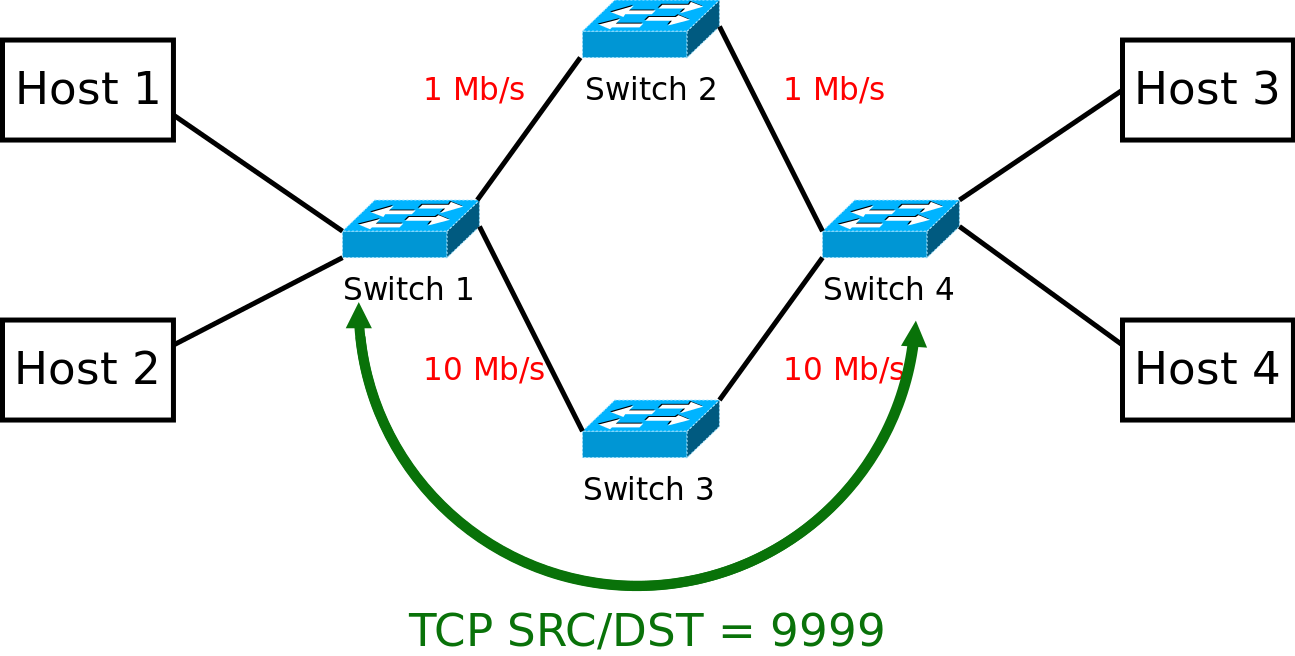
\includegraphics[width=\linewidth]{imagenes/Implementation/mininet_topology_port_slicing.png}
  \caption{Port based slices.}
  \label{fig:port_slicing}
\end{figure}

To fully understand the implementation of this scenario, we need to know how the switch ports are numbered. Every port number is shown in Table \ref{tab:switch_ports}.

\begin{table}
    \centering
    \caption{Port numbering.}
    \vspace{0.1 cm}
    \begin{tabular}{c c}
    \hline
    \rowcolor{lightgray}
    \textbf{Link (A - B)}                        &\textbf{Port number (A - B)}     \\ \hline
    Switch 1 - Host 1                            & 3 - 1                           \\ \hline 
    Switch 1 - Host 2                            & 4 - 1                           \\ \hline 
    Switch 1 - External Host 1                   & 5 - 1                           \\ \hline 
    Switch 2 - Switch 1                          & 1 - 1                           \\ \hline 
    Switch 3 - Switch 1                          & 1 - 2                           \\ \hline 
    Switch 4 - Switch 3                          & 2 - 2                           \\ \hline 
    Switch 4 - Switch 2                          & 1 - 2                           \\ \hline 
    Switch 4 - Host 3                            & 3 - 1                           \\ \hline 
    Switch 4 - Host 4                            & 4 - 1                           \\ \hline 
    Switch 4 - External Host 2                   & 5 - 1                           \\ \hline 
    \end{tabular}
    \label{tab:switch_ports}
\end{table}

We will now go through a brief overview of the necessary commands. To see the full code refer to Appendix \ref{annex:port_slicing}. First of all, we have to create two slices.
\begin{lstlisting}
    fvctl -n add-slice fast_slice tcp:localhost:10001 admin@fastSlice
    fvctl -n add-slice slow_slice tcp:localhost:10002 admin@slowSlice
\end{lstlisting}

Next, we add the flowspaces. As an example, we will show the flowspaces for switch 1.
\begin{lstlisting}
    fvctl -n add-flowspace dpid1_port3_fast_src 1 100 in_port=3,tcp_src=9999 fast=7
    fvctl -n add-flowspace dpid1_port3_fast_dst 1 100 in_port=3,tcp_dst=9999 fast=7
    fvctl -n add-flowspace dpid1_port3_slow 1 1 in_port=3 slow=7
    fvctl -n add-flowspace dpid1_port4_fast_src 1 100 in_port=4,tcp_src=9999 fast=7
    fvctl -n add-flowspace dpid1_port4_fast_dst 1 100 in_port=4,tcp_dst=9999 fast=7
    fvctl -n add-flowspace dpid1_port4_slow 1 1 in_port=4 slow=7
    fvctl -n add-flowspace dpid1_port2 1 100 in_port=2 fast=7
    fvctl -n add-flowspace dpid1_port1 1 1 in_port=1 slow=7
\end{lstlisting}

When it comes to the priorities for each flow, any priority can be used as long as the relativity between them is maintained, i.e., the higher priorities are kept higher than the lower ones.

After configuring every slice and flowspace, we just need to launch FlowVisor and two POX controllers, one listening on port 10001 and the other one on 10002. And that would be it for TCP port slicing. 

Lastly, this is just simple example to get familiar with Mininet, POX, FlowVisor and its syntax. In the next section we will tackle a more complex and involved example now that we know the very basics of network slicing.

\section{IP Address Slicing}
Now, for a more complex scenario, we are going to slice the network depending on the source and destination IP address, see Figure \ref{fig:IP_slicing}. Notice that, before we implement a new scenario, we need to remove the slices created on the previous one. Otherwise the flowspaces and slices will overlap and result on unpredictable behaviour.
\begin{figure}
  \centering
  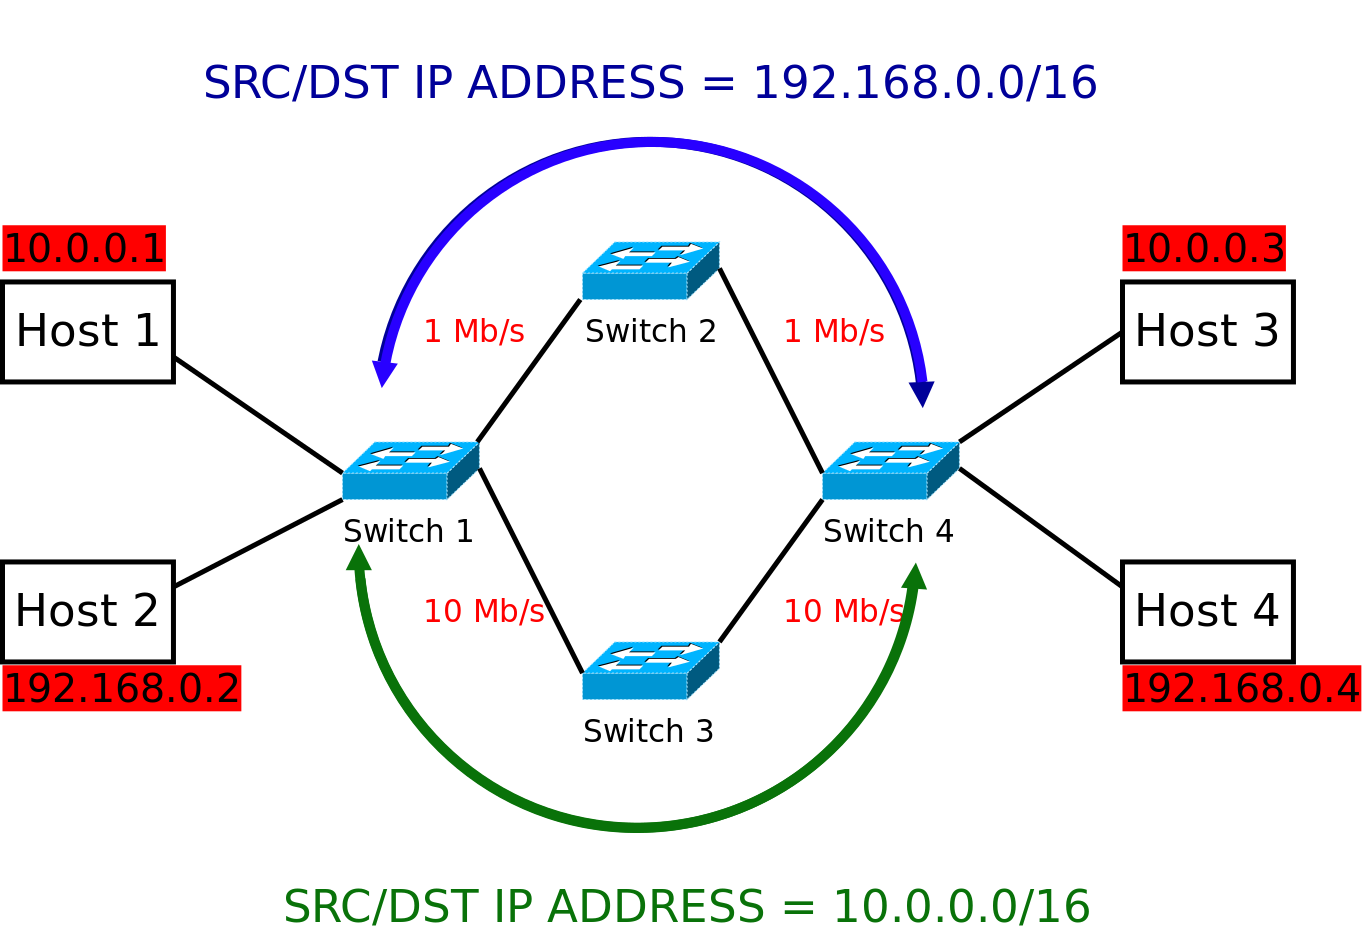
\includegraphics[width=\linewidth]{imagenes/Implementation/mininet_topology_IP_slicing.png}
  \caption{IP address based slices.}
  \label{fig:IP_slicing}
\end{figure}

Similarly to what we did in the previous example, we start by creating the slices. We want to test this scenario later using LoRa packets, thus we name the slices \textit{LoRa} and \textit{Regular}. Furthermore, given that FlowVisor does not have the option to intentionally drop packets, we will create a third slice for this purpose, \textit{DevNull}. This way, whenever we want to intentionally drop packets, we will send them to the DevNull slice. 
\begin{lstlisting}
    fvctl -n add-slice LoRa tcp:localhost:10001 admin@LoRaSlice
    fvctl -n add-slice Regular tcp:localhost:10002 admin@RegularSlice
    fvctl -n add-slice DevNull tcp:localhost:666 admin@DevNull
\end{lstlisting}

In addition, we also want to isolate both subnets, e.g., host 1 cannot communicate with host 4. This is already the case by default because we are using switches. Yet, it is possible to manually add entries to the ARP table so that the switch can route between both subnets. To prevent this, we will actively drop packets that try to leave their original subnet.

Similarly to what we did in the previous example, we will show the flowspaces for switch 1. For the full script, refer to Appendix \ref{annex:ip_slicing}. Also remember that Table \ref{tab:switch_ports} holds the information for the ports of switch 1.
\begin{lstlisting}
    fvctl -n add-flowspace dpid1_LoRa 1 100 nw_src=10.0.0.0/16 LoRa=6
    fvctl -n add-flowspace dpid1_DevNull_LoRa2Regular 1 200 nw_src=10.0.0.0/16,nw_dst=192.168.0.0/16 DevNull=2
    fvctl -n add-flowspace dpid1_DevNull_Regular2LoRa 1 200 nw_dst=192.168.0.0/16,nw_src=10.0.0.0/16 DevNull=2
    fvctl -n add-flowspace dpid1_default 1 1 any Regular=6
    fvctl -n add-flowspace dpid1_DevNull_port1_ARP 1 300 in_port=1,nw_src=10.0.0.0/16,dl_type=0x0806 DevNull=6
    fvctl -n add-flowspace dpid1_Regular_port1 1 1 in_port=1 Regular=6
    fvctl -n add-flowspace dpid1_LoRa_port2_LoRa 1 200 in_port=2,nw_src=10.0.0.0/16 LoRa=6
    fvctl -n add-flowspace dpid1_DevNull_port2 1 1 in_port=2 DevNull=2
\end{lstlisting}

The main ideas behind the flowspaces are:
\begin{itemize}
    \item Drop packets that try to travel between subnets.
    \item Assign packets with \textit{nw\_src=10.0.0.0/16} to LoRa.
    \item Assign ARP packets with \textit{nw\_src=10.0.0.0/16} to LoRa. Technically an ARP packet does not have a network source field, but FlowVisor, due to how it is implemented internally, is able to distinguish between ARP packets based on its source.
    \item Send the rest of the packets to the regular slice.
\end{itemize}

Like we did previously, we now run two POX controllers on ports 10001 and 10002. We do not run a third controller on port 666 because the point of that slice is to drop the packets.

One could think that it should be possible to just send all ARP packets through the same path and reserve the high speed path for actual data packets. The problem with that approach is that, since we are using a learning switch controller, the switches will learn the path to the different hosts through the ARP packets. As a result, the path that is not used for ARP will be completely neglected.

Moreover, we cannot allow the ARP packets to just roam freely through the network because we are using a looped topology. If we do not take care of this loop, the ARP packets will just clog the network and render it useless. 

In conclusion, the flowspaces shown above are the result of many iterations. Mainly due to learning about the different nuances of the topology, as well as the behaviour of the different packets and protocols.

